\section{Билет 22. Теорема об устранимой особой точке для гармонических функций (случай $\R^3$)}
% Затехал: Дмитрий Федоряка
 

\begin{theorem}

{\bf (об  устранимой особой точке).} 
Пусть $u(x)$ - гармоническая в $\mathring{B}_\rho(a) \subset 
\R^3$ и $u(x)=o(E(x-a))$ при $x \to a$, где $E(x) = -\frac{1}{4 \pi |x|}$. Тогда $u(x)$ можно так доопределить в точке $a$, что она будет гармонической в $B_\rho(a) = \{x: |x-a|<\rho \}$.

\end{theorem}

\textbf{Доказательство.}


\begin{enumerate}
\item{ 
	
	$u(x) = o \brs{\frac{1}{|x|}} \Leftrightarrow |x| \cdot u(x) 
	\underset{x \to 0}{\longrightarrow} 0$
}

\item{
Возьмём $r<\rho$. 
\begin{center}
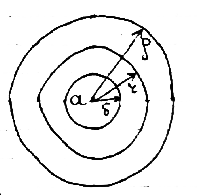
\includegraphics{22_1_new}
\end{center}
Функция $u(x)$ непрерывна на $\partial B_r (a)$.

Построим гармоническую функцию:

$$\hat{u}(x) = \frac{1}{4 \pi r} 
\oint_{|y|=r}\frac{r^2 - |x|^2}{|y-x|^3} u(y) dS_y \in 
C(|x| \le r)$$.

}


\item{

Считаем $a=0$. Покажем, что $u(x) \equiv \hat{u}(x)$ при $0<|x|\le r$. Строим $v(x) = u(x) - \hat{u}(x)$. Эта функция гармоническая в $\mathring{B}_r(a)$, непрерывная на $(0<|x| \le r)$, а также 
$v(x) \equiv 0 ~~ \forall x: |x|=r$ и $|x| \cdot v(x) \underset{x \to 0}{\longrightarrow} 0$. 
 
}

\item{

Фиксируем $\varepsilon >0$ и рассмотрим функции $W_\eps^{\pm} =
\frac{\varepsilon}{|x|} \mp v(x)$.

Функции $W_\eps^{\pm}$ также гармонические в $(0<|x|<r)$, непрерывны на $(0<|x| \le r)$, а 
$\left.W_\eps^{\pm}(x) \right|_{|x|=r} =\frac{\eps}{|x|} >0$.
}

\item{

Выберем $\delta > 0 $ так, чтобы $\forall x:~~ |x| \le \delta \to |x| \cdot |v(x)| < \frac{\varepsilon}{2}$.

При $|x|\le \delta$: 

$$
W_\varepsilon^{\pm} = \frac{\eps}{|x|} \mp v(x) \ge 
\frac{\eps}{|x|} - |v(x)|
\ge 
\frac{\eps}{|x|}\sbrs{1 - \frac{|x|\cdot |v(x)|}{\varepsilon}}
\ge
\frac{\eps}{|x|}\sbrs{1-\frac{1}{2}}
=
\frac{\varepsilon}{2|x|} >0
$$
}



\item{

При $\delta \le |x| \le r$  функции $W_\eps^{\pm}(x)$
 --- гармонические в $(\delta < |x| < r)$ и непрерывны на замыкании 
этой ограниченной области $\Rightarrow$ по принципу максимума 
максимум и минимум достигаются на границе.

Значит, $W_\varepsilon^{\pm} (x) > 0$ при $\delta \le |x| \le r$.

Итак, $W_\varepsilon^\pm(x)$ положительна в $(0<|x| \le r)$
$\Rightarrow$  $|v(x)| < \frac{\varepsilon}{|x|}$ в $(0<|x|\le r)$.

Значит, $v(x) \equiv 0$ при $0<|x|\le r$ $\Rightarrow$ $v(x)$ можно продолжить на $|x|\le r$, положив $v(0)=0$, ч.т.д. 

}

\end{enumerate}


